\chapter{Cahier de Charge} \label{CahierCharge}



\section{Définition des besoins} \label{Besoins}

\subsection{Contexte général}

Le projet SENTERRITOIRE a pour vocation la réalisation d’un site web dynamique s'appuyant sur une application existante : "TERRIDOCViewer".  L'un des objectifs de ce projet est l'enrichissement de cette dernière, notamment en y introduisant de nouvelles composantes qui permettraient d'amplifier les descripteurs, géo-spatiaux et temporels, des informations liées à l'aménagement du territoire "Montpellier Agglomération ", pour doter cette application d'une accessibilité attractive au niveau de la recherche et de la visualisation.\\

Ces informations seront extraites automatiquement à partir d'un fonds documentaire constitué de documents d'actualités sous forme de textes ; sélectionnés et analysés par des experts géographes afin d'évaluer les opinions des acteurs (exemple : Auteur d’un document choisi) quant à ces données.\\

L'objectif de ce cahier des charges est d'expliquer les grandes lignes du projet : \\

Nous préciserons, dans un premier temps, les différents besoins indispensables à la réalisation de l'application et ainsi, au rendu espéré. Nous examinerons attentivement ces derniers lors de la définition des aspects fonctionnels concernant le projet ; en avant dernière partie de ce cahier des charges.\\

Ensuite, nous évoquerons les méthodes logicielles utilisées, et concevrons une architecture appropriée au travail demandé et adaptable à TERRIDOCViewer.\\

Enfin, nous terminerons sur les aspects  techniques et ergonomiques en étudiant les points sur lesquels nous nous basons et ceux sur lesquels nous cherchons à être novateurs et soigneux. Cela grâce à des veilles et des études comparatives des différentes technologies optées et également en proposant une ergonomie que nous jugeons captivante.\\


\subsection{Composante spatiale}

L'intégration d'une composante spatiale dans l'application devra permettre de représenter et de mettre en valeur les différentes opinions dans un espace géographique sélectionné par l'utilisateur. La composante graphique devra être représentée sous la forme d'une carte de type Google Maps. \\ 

L'intégration de fonds de cartes "open source" peut s'avérer nécessaire. Selon les conditions d'utilisation de l'API GoogleMaps, l'éditeur de l'application doit acquérir une license payante à partir du moment que l'application génère plus que 25.000 cartes par jour.

La composante devra comporter toutes les fonctionnalités classique d'une application cartographie / d'un viewer cartographique (zoom etc.). L'utilisation des différentes fonctionnalités doit être intuitive et facile.


\subsubsection{Intégration de la composante opinion dans la composante spatiale}

Chaque opinion sera représentée spatialement dans la composante cartographique. La composante spatiale devra permettre de représenter ce que les acteurs pensent d'un thème donné. Il sera nécessaire de gérer le grand nombre d'informations représenté sur la carte afin de garantir une lisibilité optimale. Par exemple, à une petite échelle il n'est pas très utile d'afficher tous les thèmes sur la carte. Au contraire il peut-être intéressant de synthétiser les différentes opinion, par exemple en fonction d'un découpage administratif existant (communes, départements etc...). La représentation de l'opinion dans la composante sera donc directement liée à l'échelle d'affichage de la composante spatiale.

\subsubsection{Base de données}

L'application SENTERRITOIRE existante utilise une base de données MySQL. Néanmoins, concernant l'intégration d'une composante spatiale, il sera nécessaire de disposer d'une base de données supportant les objets géographiques et spatiaux. Il existe donc deux possibilité: Migrer la base de données existante MySQL vers une base de données PostgreSQL, pour laquelle il existe une extension spatiale.

\subsection{Composante temporelle}

La composante temporelle est outil qui doit permettre de distinguer et raffiner les informations que l'on souhaite analyser, mais aussi d'être visuellement pertinent pour en extraire des informations utiles.

Ainsi la composante temporelle doit permettre de situer un opinions dans le temps, connaître son contexte temporelle.
Elle doit aussi compléter les fonctionnalités de recherche du module en permettant à l'utilisateur d'indiquer une période ou une date, de n'afficher que les opinions relatif à cette dernière.

Le composant doit permettre également la représentation d'un opinion dans le temps, c'est à dire pouvoir constater les évolutions (positive-négative) sur une période donnée.

Étant donnée la quantités d'informations que la composante est susceptible d'afficher, elle devra posséder des outils permettant d'abstraire simplement des classes d'opinions (isoler, regrouper) parmi la masse affiché.

\section{Conception de l’architecture} \label{Architecture}

L'architecture 3-tiers convient parfaitement à ce genre d'application. Elle présente à la fois une grande fiabilité, une bonne disponibilité, une excellente évolutivité. \\

Elle permet de bien séparer l'application en trois parties distinctes :

\begin{itemize}
\item User interface : La partie présentation de l'application.
\item Business logic : La couche métier qui s'occupe du traitement de l'information. 
\item Data access : La partie accès et stockage des données.
\end{itemize}


\begin{center}
\begin{figure}[H] \centering
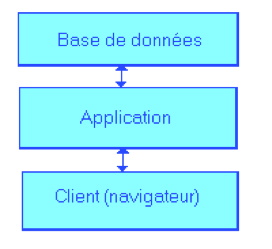
\includegraphics[width=5cm]{archi1.png}\\
\caption{\label{appli} Protocole d'échange Serveur - Employé}
\end{figure}
\end{center}

De plus, l'application existante "TERRIDOCViewer" se base sur cette architecture-là.

\textbf{Dans le cadre de ce TER, nous interviendrons principalement dans le tier "User Interface" et tout ce qui est requêtage à la Base de Données pour récupérer les informations à afficher à l’utilisateur.}

\textbf{User interface :}\\

Pour ce tier, la vue sera composée des modules suivants : 
\begin{itemize}

\item Un module de recherche opinion pour valoriser les opinions selon des thématiques données.
\item Un module de recherche spatiale qui lui, consiste en un service de cartographie en ligne style "Google Maps", pour générer une carte géographique comprenant des icônes faisant références aux opinions selon des lieux précis.
\item Un module de recherche temporelle qui consiste en une frise chronologique permettant de situer dans le temps les opinions des utilisateurs.

\end{itemize}


\textbf{Business logic}\\
Ce tier permettra de gérer les requêtes clientes et de renvoyer les données nécessaires aux clients en réponses à leurs requêtes. Il sera basé sur  le pattern MVC : Modèle, Vue et Contrôleur comme pour l'application existante.


\textbf{Data access}\\

Ce tier aura pour but principal de stocker des informations de type géolocalisation, des informations temporelles et les opinions des utilisateurs concernant une thématique donnée.

Pour rester dans la même optique que l'application existante,  nous reprendrons l’architecture 3-tiers de la thèse de Monsieur KERGOSIEN dont le tier "Business logic" est basé sur le pattern MVC.


\begin{center}
\begin{figure}[H] \centering
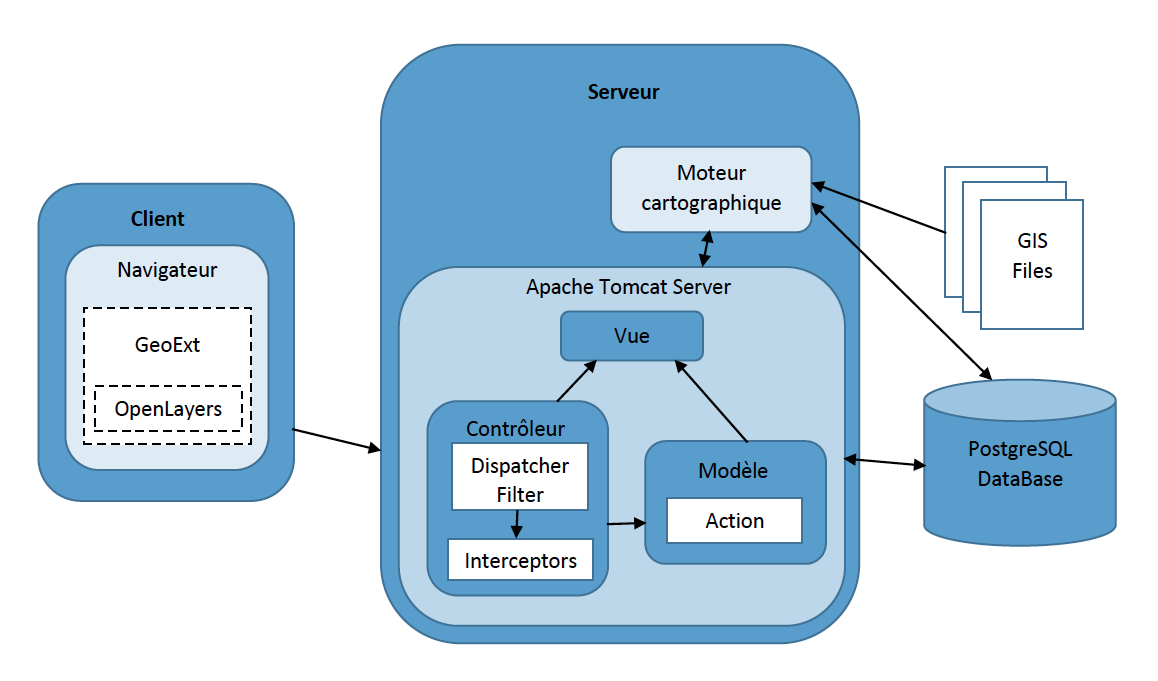
\includegraphics[width=19cm]{archi2.png}\\
\caption{\label{archi2} Architecture 3-tiers}
\end{figure}
\end{center}


\section{Définition des aspects fonctionnels} \label{Fonctionnels}

\subsection{Composante spatiale}

La composante spatiale sera lié dynamiquement à l'arborescence des thématiques et à la composante temporelle. Par exemple, lorsqu'un utilisateur sélectionne un thème dans l'arborescence des thématiques les opinions représentés sur la carte sont mis à jour de façon dynamique (les  thèmes non-sélectionnées ne seront plus affichés). La composante spatiale devra comporter les fonctionnalités suivantes :

\begin{itemize}

\item Intégration de différentes couches de fonds de cartes (vues satellites, vue plan etc.)
\item Zoom(s)
\item Déplacement
\item Interrogation d'objets (par exemple un point représentant un thème)
\item Sélection de l'échelle souhaité
\item Calcul de distance et de surface
\item Sélection / dé-sélection d'informations (par exemple afficher seulement points mais pas l'opinion).
\end{itemize}  


Nous allons nous focaliser sur deux méthodes pour représenter les opinions sur la carte. A une échelle plus grande, les différentes thème sont représentés sous forme d'icônes (ou de points) et l'utilisateur peut cliquer sur l'icône pour visualiser les opinions par rapport à ce thème bien précis. Au contraire, à une échelle plus petite, il peut être envisagé d'utiliser les découpages administratifs existants (par exemple départements, régions ou quartiers de ville) afin de hiérarchiser l'opinion moyenne sur un territoire géographique donné. Des requêtes sur les informations stockées dans la base de données permettront d'extraire ce genre d'information.


\subsubsection{Base de données}

La nouvelle base de données devra permettre de récupérer facilement et rapidement les informations spatiales / géographiques liées à un terme ou à une opinion. Il aurait été possible de conserver la base de données MySQL existante mais comme il n'existe pas d'extension spatiale performante pour ce type de base de données, il aurait été nécessaire de gérer simultanément deux bases de données différentes. Cependant il est plus intéressant de migrer la base de données existante vers une base de données PostgreSQL afin de faciliter la gestion et la programmation de l'application.



\subsubsection{Composante temporelle}

 D'après l'analyse des besoins, l'outil visuel qui correspond aux plus près des besoins de la composante temporelle est une frise. C'est un outil efficace qui permet d'abstraire facilement des informations sur un sujet dans le temps. \\
 
«Une frise chronologique ou ligne du temps est une représentation linéaire d’événements positionnés sur la flèche du temps; elle associe des événements à leurs positions dans le temps le long d'une échelle graduée, ce en quoi elle se rapproche d'une chronologie.»\\

Nous souhaitons indexer et montrer l’évolution des thématiques d'opinions dans le temps avec un outil visuel ergonomique et efficace. La frise chronologique remplie ces propriétés :\\

\begin{itemize}

\item La composante développé doit permettre une manipulation dynamique de la frise chronologique et s'intégrer ergonomiquement dans le module.
\item On doit pouvoir naviguer chronologiquement, c'est à dire faire glisser la frise pour faire défiler les dates.
\item On souhaite aussi avoir la possibilité de spécifier l'échelle du temps. Par exemple sur une période qui nous intéresse, l'utilisateur doit pouvoir zoomer pour afficher plus de détail, ou au contraire dé-zoomer.
\item La frise doit mettre à disposition des outils pour manipuler les thématiques à afficher. Les outils de sélection doivent permettre de pouvoir spécifier, généraliser ou regrouper des thématiques dans le but que l'utilisateur puissent composer facilement avec les éléments qui l'intéresse.
\end{itemize}



\section{Définition des aspects techniques et ergonomiques} \label{Technique}

<<<<<<< HEAD
\subsection{Composante spatiale}
=======
\section{Composante temporelle}
Après quelques recherche, il n'y a pas de solution qui correspondent à toutes les exigences réunit d'après la description fonctionnelle. Il faut donc prévoir de développer tout ou des parties de la composantes temporelle.
Une première approche est de récupérer le code d'une frise qui se rapproche le plus des spécifications imposer et développer les fonctionnalités qu'il manque. Problème il faut comprendre le code. On est pas sure d'y arriver. De plus d'un point de vue pédagogique, pas de capitalisation de compétence sur les techniques moderne d' ingénierie logiciel (api, framework).
La second option est de développer la composante à l'aide d'une api ou d'un framework. L'application actuelle est développé à l'aide du framework extjs. Il est donc cohérent d'utiliser le extjs afin de respect une cohérence dans le développement de l'application. De plus extjs est un framework très populaire et largement documenté. D'un point de vue technique extjs possède un librairie d'objet qui permettre diverse solution pour la manipulation des données json.

\section{Composante spatiale}

Pour la composante spatiale, nous avons décidé d'intégrer un serveur cartographique dans l'application. Le serveur va générer la carte en fonction des choix effectués par l'utilisateur. Ceci nous permettra de gérer dynamiquement la composante spatiale de l'application. Ce serveur permettre d'afficher des données géographiques sous forme vectorielle ou cartographique. Pour ce type de serveur, il existe trois possibilités : MapServer et GeoServer.

>>>>>>> 41f60650e227153521f5419a98853a338d79012a

Pour la composante spatiale, nous avons décidé d'intégrer un moteur cartographique dans l'application. Le serveur va générer la carte en fonction des choix effectués par l'utilisateur. Ceci nous permettra de gérer dynamiquement la composante spatiale de l'application. Ce serveur permettra d'afficher des données géographiques sous forme vectorielle ou cartographique. Pour ce type de moteur, nous allons comparer deux types de logiciels : Geoserver et Mapserver. 

\paragraph{Comparaison}

\subparagraph{Mapserver}
Mapserver est un moteur cartographique OpenSource qui permet de générer des cartes de manière dynamique et d'effectuer des requêtes dans une base de données spatiale. Mapserver a été écrit en C, est multi-plateforme et fait partie de la fondation OsGeo. Différentes sources données sont supportées : \\

\begin{itemize}

\item Raster (Tiff, GeoTiff, PNG, etc.)
\item Vecteur (ESRI shapefile, Base de données spatiale (PostGIS etc.)
\item Service Web OGC (WFS, WMS ...)

\end{itemize}

Mapserver fonctionne avec CGI. L'administration des services est fait via des "mapfile" dans lesquels ont peut également définir l'habillage des cartes. Les performances d'habillage restent cependant très limités. \\

\subparagraph{Geoserver}
Geoserver est un projet de moteur cartographique plus récent (fonée en 2003). Geoserver a été développé en Java et est également multi-platforme. Geoserver supporte les mêmes formats de données que Mapserver (la seule différences est qu'il supporte également des services WFS-T). L'administration des services est effectuée via une interface d'administration ce qui facilite considérablement l'utilisation et la prise en main de ce moteur cartographique. Geoserver utilise du J2EE. \\


A l'instant nous ne savons pas quel moteur cartographique nous allons utiliser. Les deux moteurs présentent peu de différences et il reste à voir avec les différents encadrant quel moteur sera le plus compatible. Aussi faudra-t-il prendre en compte l'hébergement de l'application. \\

\paragraph{Habillage de la carte}

Par rapport à l'habillage de la carte (bouttons pour zoomer, choix de l'échelel etc.) nous avons décidé de choisir GeoExt, ExtJS et OpenLayers. \\

OpenLayers est une API disponible sous licence libre qui propose différents composant pour créer des cartes dynamiques. Le code est exécuté entièrement côté client par le navigateur.\\

GeoExt, tout comme ExtJS, fournit un ensemble de composants JavaScript graphiques (Widgets) prêts à l’emploi. La documentation d'API et de nombreux exemples sont disponibles sur le site. L'objectif principal de GeoEXT est de faciliter le couplage entre OpenLayers et ExtJS. Voici quelques exemples d'utilisation de GeoExt qui vont être utile pour l'élaboration de cette application: 

\begin{itemize}
\item Afficher un popup ExtJS au moment du clic sur un objet de la carte
\item Structure arborescente ExtJS contenant les couches OpenLayers
\item Création de barres (slider) ExtJS pour régler la transparence d'une couche OpenLayers
\item Afficher une liste déroulante ExtJS contenant les échelles d'affichage disponibles pour la carte OpenLayers.
\end{itemize}

\subsection{Base de données}

PostGIS est une extension du système de gestion de base de données PostgreSQL qui permet de gérer (stocker, manipuler) des données (objets) géographiques dans une base de données. Cette extension permet d'utiliser une base de données PostgreSQL comme
une base de données dans n'importe quel projet SIG. Depuis la dernière version PostGIS 2.0, PostGIS gère les données raster (données images). PostGIS est compatible avec des nombreux autres outils, notamment QGIS, Mapserver ou Geoserver.
PostgreSQL / PostGIS sera le SGBD idéal pour répondre aux besoins de l'application.

\section{Composante temporelle}
Après quelques recherche, il n'y a pas de solution qui correspondent à toutes les exigences réunit d'après la description fonctionnelle. Il faut donc prévoir de développer tout ou des parties de la composantes temporelle.

Une première approche est de récupérer le code d'une frise qui se rapproche le plus des spécifications imposer et développer les fonctionnalités qu'il manque. Problème il faut comprendre le code. On est pas sure d'y arriver. De plus d'un point de vue pédagogique, pas de capitalisation de compétence sur les techniques moderne d' ingénierie logiciel (api, framework).

La second option est de développer la composante à l'aide d'une api ou d'un framework. L'application actuelle est développé à l'aide du framework extjs. Il est donc cohérent d'utiliser le extjs afin de respect une cohérence dans le développement de l'application. De plus extjs est un framework très populaire et largement documenté. D'un point de vue technique extjs possède un librairie d'objet qui permettre diverse solution pour la manipulation des données json.


\section{Composante opinion}

Nous  proposons pour cette composante une méthode de travail assez claire qui permet l’échange de données liées aux opinions entre la base de données, la partie serveur et la partie client : \\


\begin{itemize}

\item Utiliser des requêtes SQL pour extraire les noms des attributs (o\_pos, o\_neutre et o\_neg) ainsi que leurs valeurs à partir des tables 'OpinionActeurParagraphe' et 'OpinionActeurPhrase' de la base de données SENTERRITOIRE. 

\item Utiliser le format de données Json pour récupérer le résultat des requêtes SQL. Ce format permet une plus grande vitesse de traitement, une simplicité de mise en œuvre, sans avoir besoin de parser un fichier XML pour extraire les informations car Json est reconnu nativement par Javascript.\\ 

\end{itemize}

Ce format permet également de décomposer ces informations en utilisant deux éléments structurels :


\begin{itemize}

\item   des ensembles de paires nom / valeur ;
\item   des listes ordonnées de valeurs. \\

\end{itemize}

Ces éléments comprennent 3 types de données :

\begin{itemize}

\item   des objets ;
\item   des tableaux ;
\item   des valeurs génériques de type tableau, objet, booléen, nombre, chaîne ou null.\\

\end{itemize}

\textbf{L'utilisation du format :} Il y a trois aspects: le traitement par le navigateur, par le serveur, et la transmission des données entre les deux:



\textbf{Coté client} : C'est particulièrement simple JSON faisant partie de la norme JavaScript. Le contenu d'un fichier JSON, ou la définition de données dans ce format sont assignés à une variable, laquelle devient un objet du programme.



\textbf{Coté serveur }: Les fichiers au format JSON s'utilisent dans différents langages de programmation, notamment Java grâce à des parseurs qui permettent d'accéder au contenu, et éventuellement de le convertir en classes et attributs, dans ce langage.

\textbf{L'échange de données }: La récupération d'un fichier peut se faire à partir de JavaScript de plusieurs façons:
\begin{itemize}

\item inclusion directe du fichier dans la page HTML au même titre qu'un fichier .js de JavaScript.
\item chargement par une commande JavaScript.
\item emploi de XMLHttpRequest.


\end{itemize}
Le fichier JSON est parsé par la fonction JavaScript eval().Le transfert d'un fichier au serveur se fait par XMLHttpRequest. Le fichier au format texte est traité par le parseur du langage de programmation utilisant le fichier.


\subsection{Quelques maquettes}

\begin{center}
\begin{figure}[H] \centering
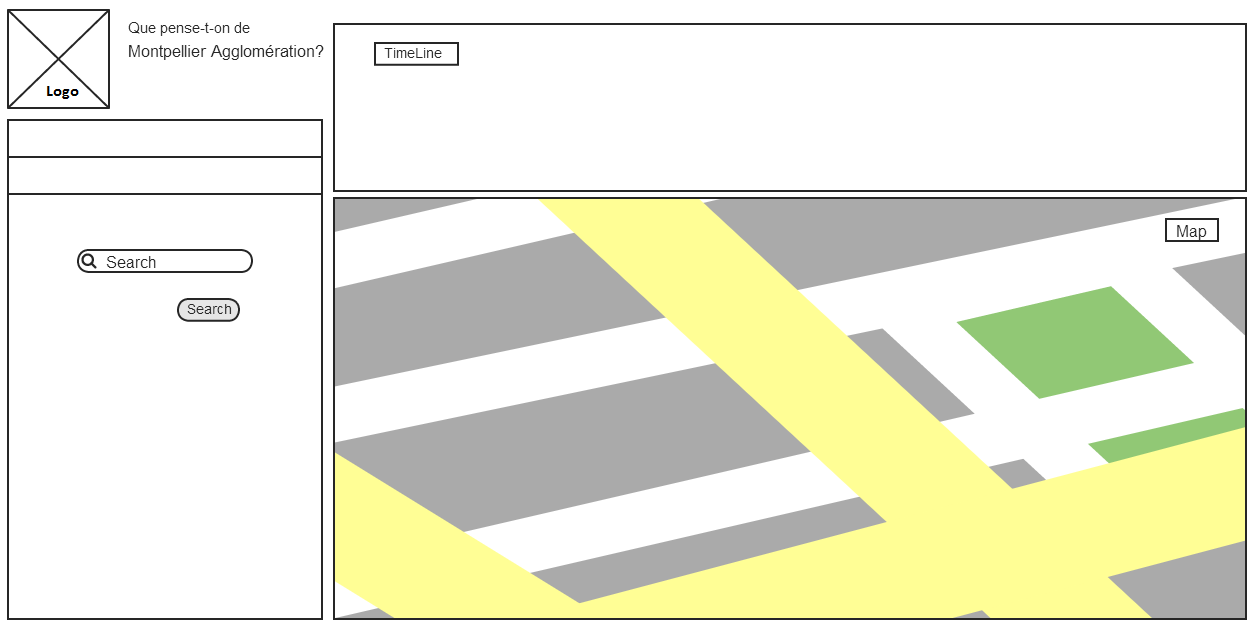
\includegraphics[width=17cm]{maquette_1.png}\\
\caption{\label{archi2} Proposition maquette 1}
\end{figure}
\end{center}

\begin{center}
\begin{figure}[H] \centering
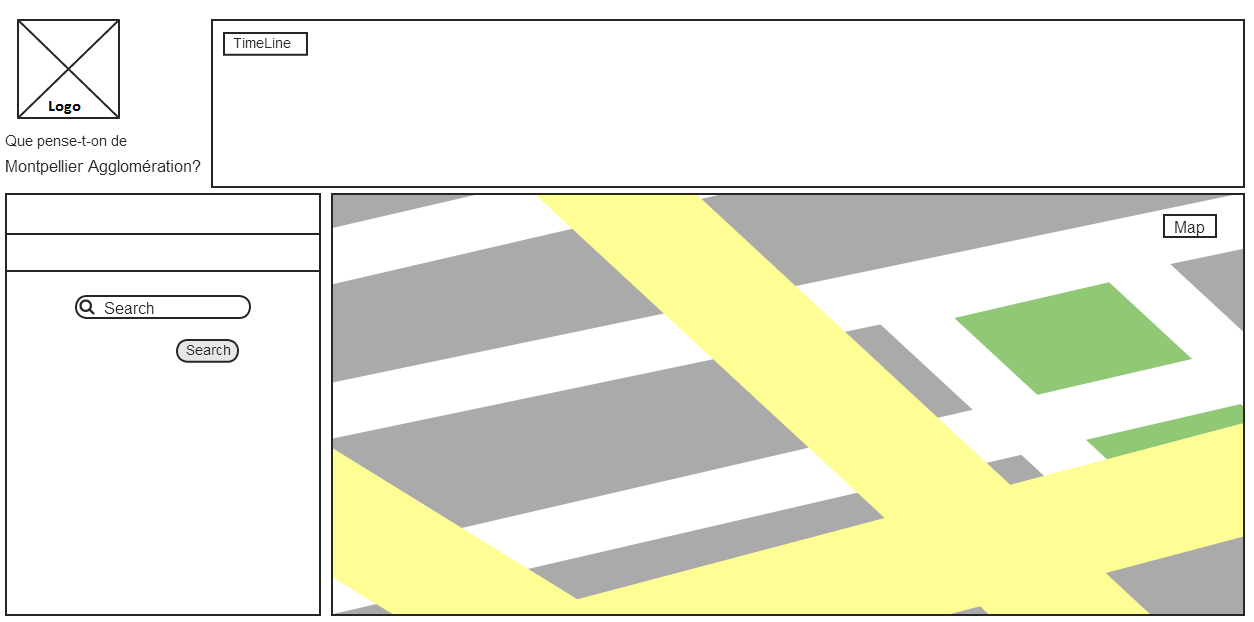
\includegraphics[width=17cm]{maquette_2.png}\\
\caption{\label{archi2} Proposition maquette 2}
\end{figure}
\end{center}

\begin{center}
\begin{figure}[H] \centering
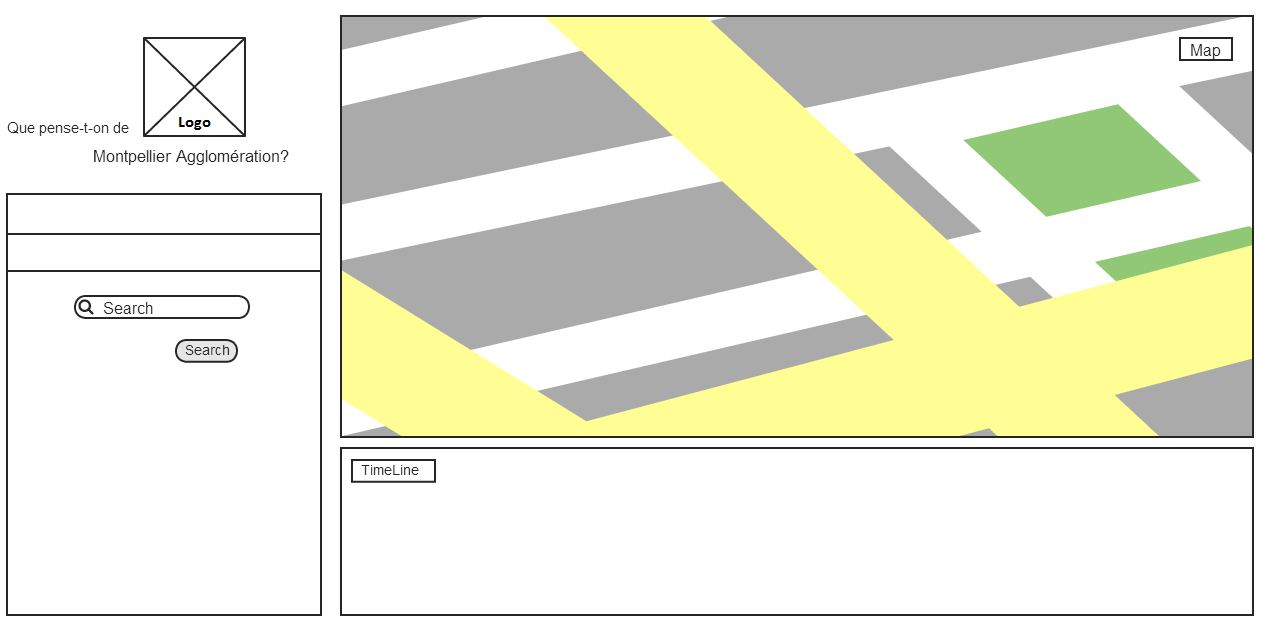
\includegraphics[width=17cm]{maquette_3.png}\\
\caption{\label{archi2} Proposition maquette 3}
\end{figure}
\end{center}
